\documentclass[a4paper,11pt]{article}

% Kodovani (cestiny) v dokumentu: utf-8
%\usepackage[cp1250]{inputenc}	% Omezena stredoevropska kodova stranka, pouze MSW.
\usepackage[utf8]{inputenc}	% Doporucujeme pouzivat UTF-8 (unicode).

\usepackage[margin=2cm]{geometry}
\newtoks\jmenopraktika \newtoks\jmeno \newtoks\datum
\newtoks\obor \newtoks\skupina \newtoks\rocnik \newtoks\semestr
\newtoks\cisloulohy \newtoks\jmenoulohy
\newtoks\tlak \newtoks\teplota \newtoks\vlhkost

\jmenopraktika={Fyzikální praktikum 2}
\jmeno={Lukáš Lejdar}
\datum={10. ledna 2024}
\obor={F}
\skupina={Út 16:00}

\cisloulohy={4}
\jmenoulohy={Brownův pohyb}

\tlak={100{,}5}
\teplota={21,3}
\vlhkost={46}


%%%%%%%%%%% Uzitecne balicky:
\usepackage[czech]{babel}
\addto\captionsczech{\renewcommand{\figurename}{Graf}}

\usepackage{graphicx}
\usepackage{amsmath}
\usepackage{xspace}
\usepackage{url}
\usepackage{indentfirst}
\usepackage{wrapfig}
\usepackage{xcolor}
\usepackage{subfig}
\usepackage{subcaption}
\usepackage{enumitem}
\usepackage{tikzsymbols}
\usepackage{newfloat}

\DeclareFloatingEnvironment[fileext=lof]{graph}
\captionsetup[graph]{labelformat=simple, labelsep=colon, name=Graf}

%%%%%% Zamezeni parchantu:
\widowpenalty 10000 \clubpenalty 10000 \displaywidowpenalty 10000
%%%%%% Parametry pro moznost vsazeni vetsiho poctu obrazku na stranku
\setcounter{topnumber}{3}	  % max. pocet floatu nahore (specifikace t)
\setcounter{bottomnumber}{3}	  % max. pocet floatu dole (specifikace b)
\setcounter{totalnumber}{6}	  % max. pocet floatu na strance celkem
\renewcommand\topfraction{0.9}	  % max podil stranky pro floaty nahore
\renewcommand\bottomfraction{0.9} % max podil stranky pro floaty dole
\renewcommand\textfraction{0.1}	  % min podil stranky, ktery musi obsahovat text
\intextsep=8mm \textfloatsep=8mm  %\intextsep pro ulozeni [h] floatu a \textfloatsep pro [b] or [t]

% Tecky za cisly sekci:
\renewcommand{\thesection}{\arabic{section}.}
\renewcommand{\thesubsection}{\thesection\arabic{subsection}.}
% Jednopismenna mezera mezi cislem a nazvem kapitoly:
\makeatletter \def\@seccntformat#1{\csname the#1\endcsname\hspace{1ex}} \makeatother
%
\newcommand{\vsn}[4]{\ensuremath{#1 =} #2(#3)\,#4}
\newcommand{\vrn}[6]{\ensuremath{#1 =} (#2 $\pm$ #3)\,#4 ($p=$ #5\,\%, $\nu=$ #6)}

\newcommand*\circled[1]{\tikz[baseline=(char.base)]{
		\node[shape=circle,draw,inner sep=1pt] (char) {#1};}}

%%%%%%%%%%%%%%%%%%%%%%%%%%%%%%%%%%%%%%%%%%%%%%%%%%%%%%%%%%%%%%%%%%%%%%%%%%%%%%%
% Zacatek dokumentu
%%%%%%%%%%%%%%%%%%%%%%%%%%%%%%%%%%%%%%%%%%%%%%%%%%%%%%%%%%%%%%%%%%%%%%%%%%%%%%%

\begin{document}

\thispagestyle{empty}

{
\begin{center}
\sf 
{\Large Ústav fyziky a technologií plazmatu Přírodovědecké fakulty Masarykovy univerzity} \\
\bigskip
{\huge \bfseries FYZIKÁLNÍ PRAKTIKUM} \\
\bigskip
{\Large \the\jmenopraktika}
\end{center}

\bigskip

\sf
\noindent
\setlength{\arrayrulewidth}{1pt}
\begin{tabular*}{\textwidth}{@{\extracolsep{\fill}} l l}
\large {\bfseries Zpracoval:}  \the\jmeno & \large  {\bfseries Naměřeno:} \the\datum\\[2mm]
\large  {\bfseries Obor:} \the\obor  \hspace{40mm}  {\bfseries Skupina:} \the\skupina %
&\large {\bfseries Testováno:}\\
\\
\hline
\end{tabular*}
}

\bigskip

{
\sf
\noindent \begin{tabular}{p{4cm} p{0.6\textwidth}}
\Large  Úloha č. {\bfseries \the\cisloulohy:} \par
\smallskip
$T=\the\teplota$~$^\circ$C \par
$p=\the\tlak$~kPa \par
$\varphi=\the\vlhkost$~\%
&\Large \bfseries \the\jmenoulohy  \\[2mm]
\end{tabular}
}

\vskip1cm

\section{Úvod}
 
\section{Postup měření}



\begin{equation}
    \langle x^2 \rangle = \frac{2RT}{6 \pi \nu r N_A}t
\end{equation}

\begin{equation}
\langle L^2_{t} \rangle = \frac{\sum_{i=0}^{n-t} L^2_{i, i+t}}{n-t}, \quad  \text{pro } t = 1,2,3 \text{ s}
\end{equation}

\begin{equation*}
 \langle L_5^2 \rangle : \langle L_{10}^2 \rangle : \langle L_{15}^2 \rangle = 1 : 2 : 3
\end{equation*}

\newpage

\section{Výsledky měření}

\begin{figure}[htpb]
    \centering
    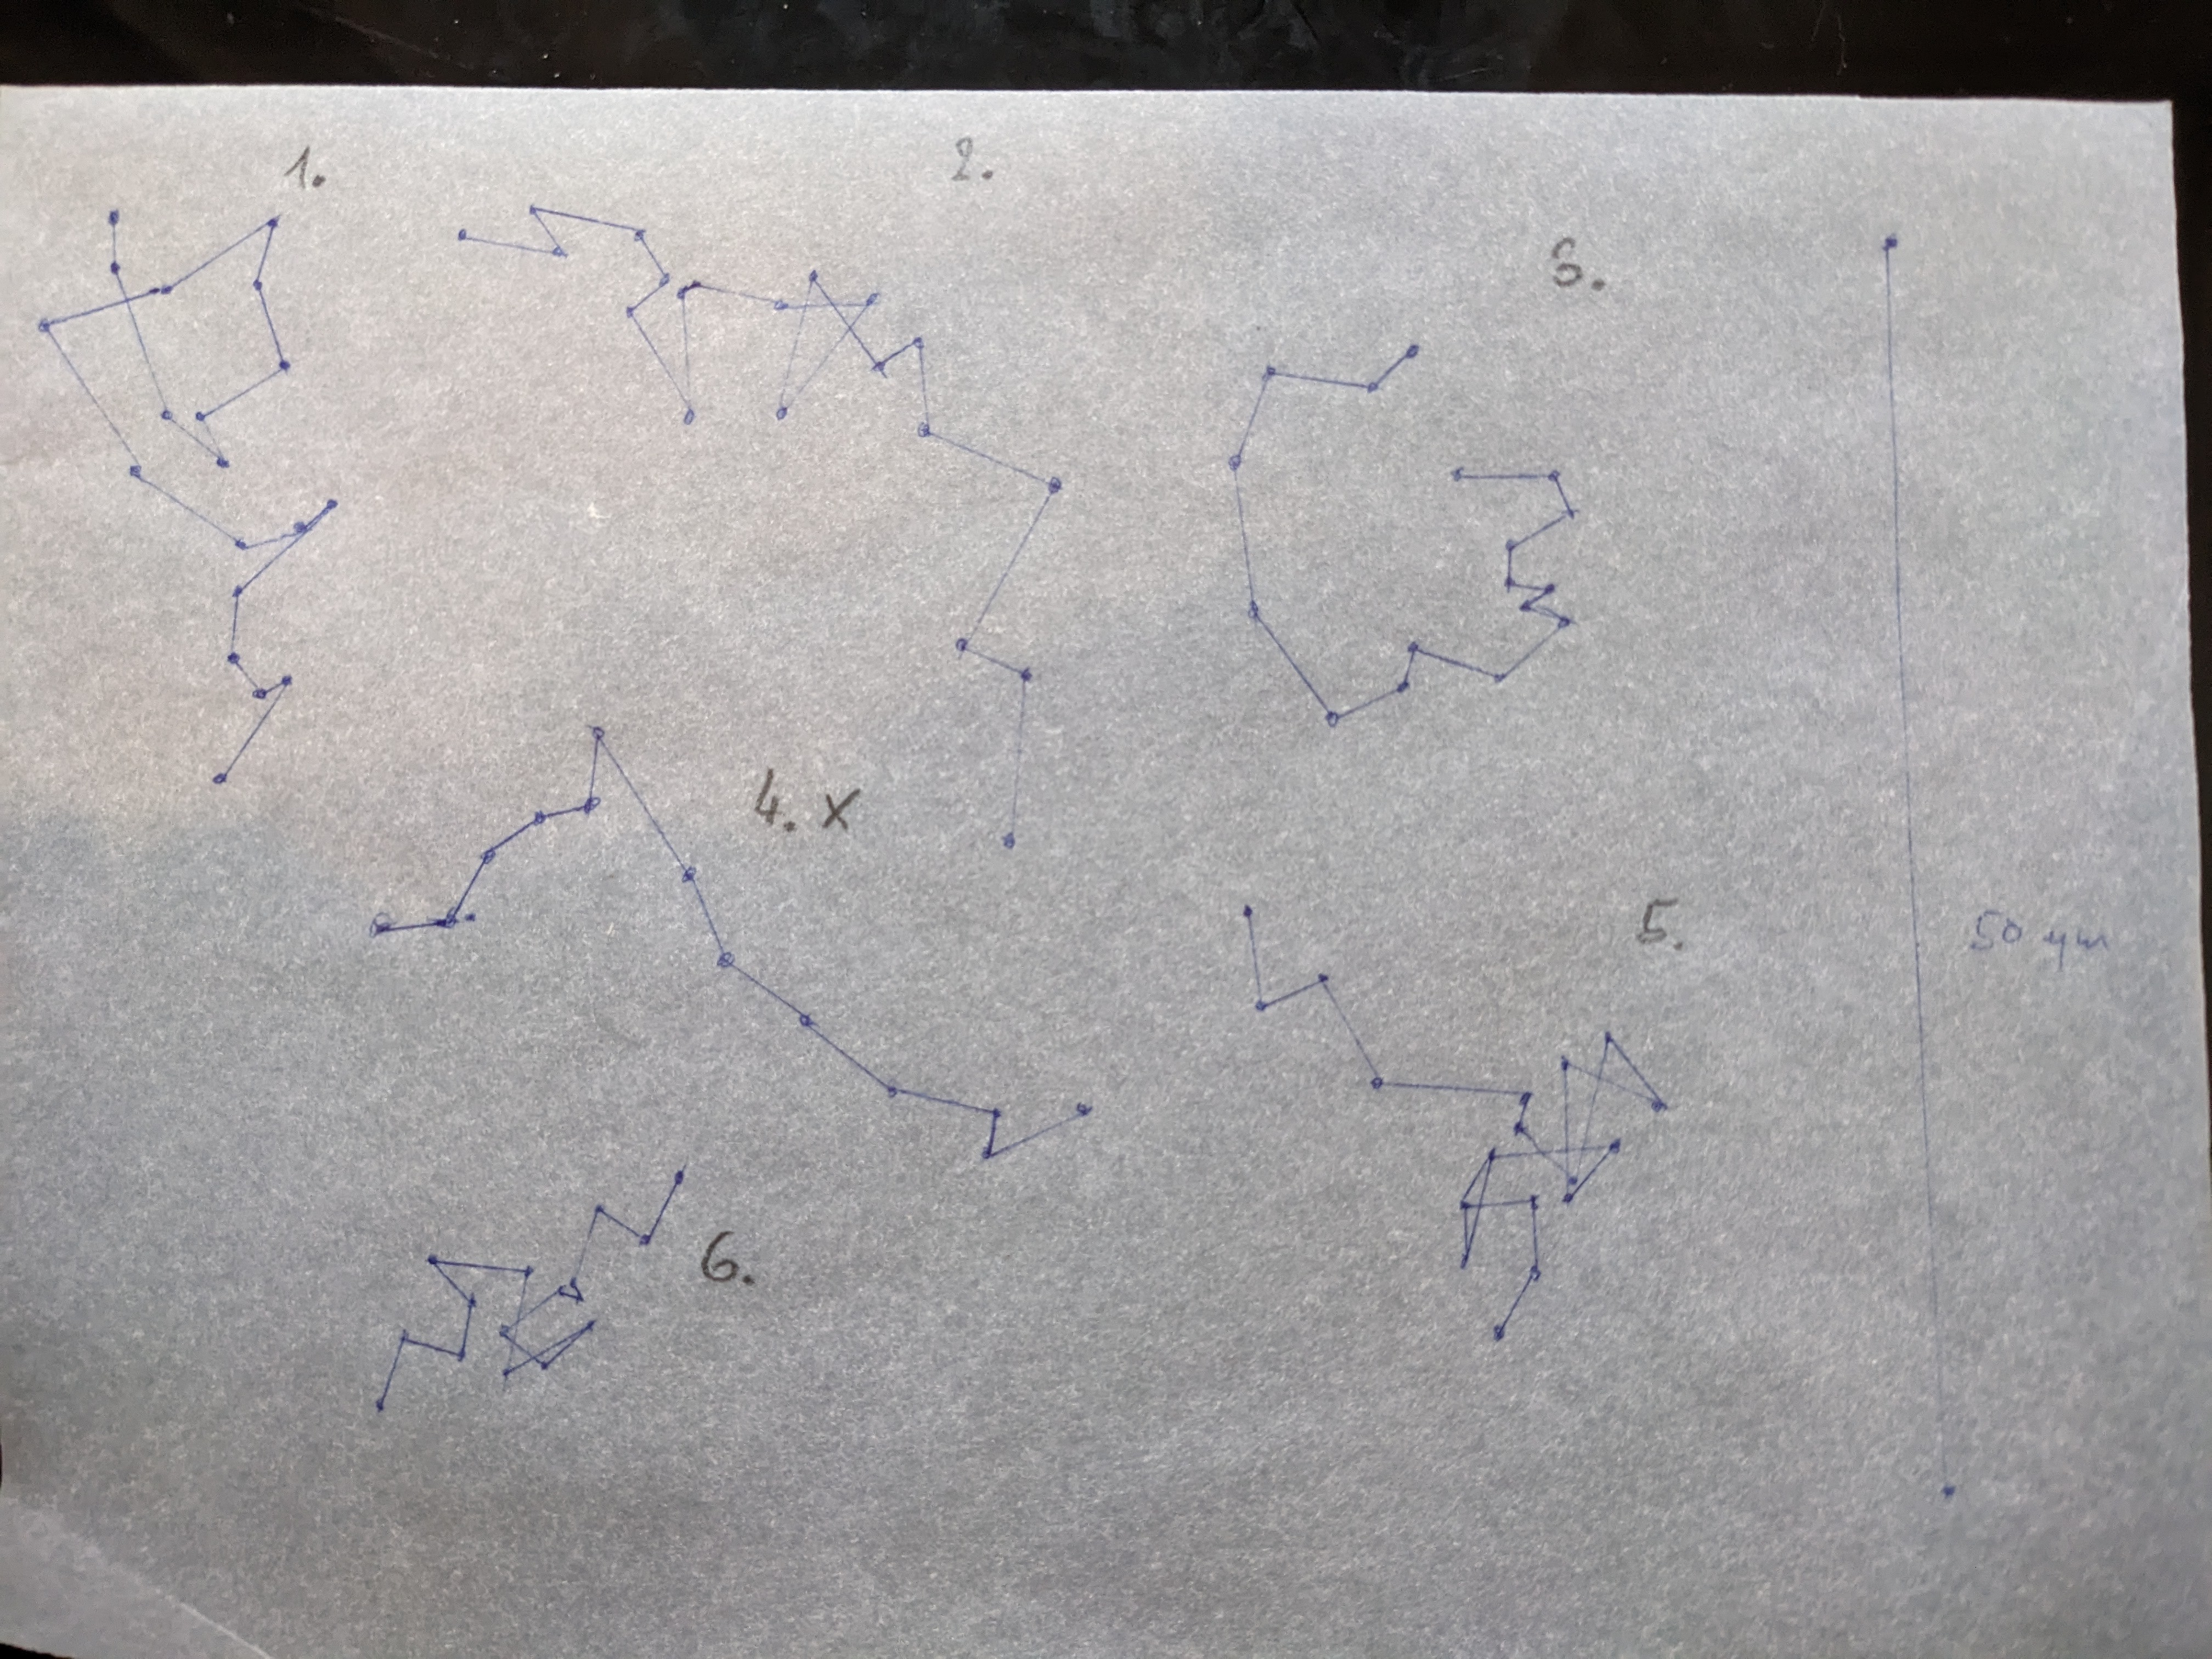
\includegraphics[trim=10 250 100 200, clip, width=0.7\textwidth]{brown_pct2.jpg}
    \caption{}
\end{figure}

\begin{table}[htpb]
    \centering
    \scriptsize
    \begin{tabular}{c | r r | r r | r r | r r | r r | c}
        \multicolumn{1}{r|}{$ t $ (s)} & $ x_1 $ & $ y_1 $ & $ x_2 $ & $ y_2 $ & $ x_3 $ & $ y_3 $ & $ x_5 $ & $ y_5 $ & $ x_6 $ & $ y_6 $ & průměr  \\
        \hline\hline
       \multicolumn{1}{r|}{  5} & 62  & 128 & 251 & 135 & 766 & 188 & 678 & 459 & 209 & 699 &  \\
       \multicolumn{1}{r|}{ 10} & 63  & 152 & 303 & 143 & 744 & 206 & 685 & 505 & 221 & 667 &  \\
       \multicolumn{1}{r|}{ 15} & 91  & 223 & 288 & 123 & 689 & 199 & 719 & 491 & 252 & 675 &  \\
       \multicolumn{1}{r|}{ 20} & 120 & 245 & 346 & 134 & 669 & 242 & 749 & 542 & 258 & 650 &  \\
       \multicolumn{1}{r|}{ 35} & 108 & 222 & 361 & 156 & 680 & 312 & 829 & 548 & 236 & 630 &  \\
       \multicolumn{1}{r|}{ 40} & 154 & 198 & 341 & 171 & 723 & 364 & 826 & 563 & 288 & 635 &  \\
       \multicolumn{1}{r|}{ 55} & 140 & 159 & 374 & 222 & 762 & 350 & 855 & 588 & 276 & 683 &  \\
       \multicolumn{1}{r|}{ 60} & 148 & 129 & 370 & 161 & 767 & 331 & 875 & 519 & 322 & 660 &  \\
       \multicolumn{1}{r|}{ 75} & 91  & 162 & 377 & 158 & 814 & 345 & 903 & 551 & 297 & 681 &  \\
       \multicolumn{1}{r|}{ 80} & 25  & 179 & 422 & 168 & 849 & 318 & 851 & 532 & 275 & 664 &  \\
       \multicolumn{1}{r|}{ 95} & 73  & 249 & 472 & 165 & 828 & 310 & 852 & 596 & 305 & 644 &  \\
       \multicolumn{1}{r|}{100} & 131 & 285 & 424 & 219 & 841 & 302 & 878 & 571 & 316 & 648 &  \\
       \multicolumn{1}{r|}{115} & 163 & 276 & 440 & 154 & 819 & 299 & 811 & 577 & 312 & 640 &  \\
       \multicolumn{1}{r|}{120} & 180 & 264 & 476 & 197 & 819 & 281 & 797 & 626 & 326 & 605 &  \\
       \multicolumn{1}{r|}{135} & 129 & 307 & 498 & 185 & 852 & 265 & 796 & 600 & 351 & 619 &  \\
       \multicolumn{1}{r|}{140} & 127 & 339 & 501 & 227 & 842 & 248 & 834 & 598 & 370 & 589 &  \\
       \multicolumn{1}{r|}{155} & 142 & 356 & 572 & 254 & 790 & 248 & 835 & 631 &     &     &  \\
       \multicolumn{1}{r|}{160} & 156 & 350 & 522 & 330 & 815 & 661 &     &     &     &     &  \\
       \multicolumn{1}{r|}{165} &     &     & 557 & 344 &     &     &     &     &     &     &  \\
       \multicolumn{1}{r|}{170} &     &     & 549 & 425 &     &     &     &     &     &     &  \\\hline\hline

       $ \langle L_5^2  \rangle \ \mu \text{m}^2 $ & 9.679 & 9.209 & 7.687 & 8.452 & 5.962 & 5.586 & 9.096 & 8.974 & 4.499 & 3.857 & 7.300 \\
       $ \langle L_{10}^2  \rangle \ \mu \text{m}^2 $ & 24.38 & 28.04 & 14.12 & 79.71 & 17.05 & 17.54 & 20.87 & 9.430 & 7.354 & 5.228 & 15.20 \\
       $ \langle L_{15}^2  \rangle \ \mu \text{m}^2 $ & 35.37 & 42.17 & 21.89 & 12.97 & 27.64 & 32.58 & 36.41 & 16.07 & 9.826 & 8.752 & 24.37 \\\hline
       $ \langle L_{10}^2 \rangle $ / $ \langle L_5^2 \rangle $ & 2.518 & 3.045 & 1.836 & 0.943 & 2.86 & 3.14 & 2.294 & 1.051 & 1.635 & 1.355 & 2.068 \\
       $ \langle L_{15}^2 \rangle $ / $ \langle L_5^2 \rangle $ & 3.654 & 4.580 & 2.847 & 1.534 & 4.637 & 5.833 & 4.003 & 1.790 & 2.184 & 2.269 & 3.333 \\
       \hline\hline
\end{tabular}
\caption{Zaznamenané souřadnice pěti různých částic, odečtené z fotky v pixelech. Měřítko je 50 $ \mu \text{m} $ : 606.1 px. }
\end{table}

\begin{equation*}
 \langle L_5^2 \rangle : \langle L_{10}^2 \rangle : \langle L_{15}^2 \rangle = 1 : 2.068 : 3.333
\end{equation*}

\begin{figure}[htpb]
    \centering
    % GNUPLOT: LaTeX picture with Postscript
\begingroup
  \makeatletter
  \providecommand\color[2][]{%
    \GenericError{(gnuplot) \space\space\space\@spaces}{%
      Package color not loaded in conjunction with
      terminal option `colourtext'%
    }{See the gnuplot documentation for explanation.%
    }{Either use 'blacktext' in gnuplot or load the package
      color.sty in LaTeX.}%
    \renewcommand\color[2][]{}%
  }%
  \providecommand\includegraphics[2][]{%
    \GenericError{(gnuplot) \space\space\space\@spaces}{%
      Package graphicx or graphics not loaded%
    }{See the gnuplot documentation for explanation.%
    }{The gnuplot epslatex terminal needs graphicx.sty or graphics.sty.}%
    \renewcommand\includegraphics[2][]{}%
  }%
  \providecommand\rotatebox[2]{#2}%
  \@ifundefined{ifGPcolor}{%
    \newif\ifGPcolor
    \GPcolorfalse
  }{}%
  \@ifundefined{ifGPblacktext}{%
    \newif\ifGPblacktext
    \GPblacktexttrue
  }{}%
  % define a \g@addto@macro without @ in the name:
  \let\gplgaddtomacro\g@addto@macro
  % define empty templates for all commands taking text:
  \gdef\gplbacktext{}%
  \gdef\gplfronttext{}%
  \makeatother
  \ifGPblacktext
    % no textcolor at all
    \def\colorrgb#1{}%
    \def\colorgray#1{}%
  \else
    % gray or color?
    \ifGPcolor
      \def\colorrgb#1{\color[rgb]{#1}}%
      \def\colorgray#1{\color[gray]{#1}}%
      \expandafter\def\csname LTw\endcsname{\color{white}}%
      \expandafter\def\csname LTb\endcsname{\color{black}}%
      \expandafter\def\csname LTa\endcsname{\color{black}}%
      \expandafter\def\csname LT0\endcsname{\color[rgb]{1,0,0}}%
      \expandafter\def\csname LT1\endcsname{\color[rgb]{0,1,0}}%
      \expandafter\def\csname LT2\endcsname{\color[rgb]{0,0,1}}%
      \expandafter\def\csname LT3\endcsname{\color[rgb]{1,0,1}}%
      \expandafter\def\csname LT4\endcsname{\color[rgb]{0,1,1}}%
      \expandafter\def\csname LT5\endcsname{\color[rgb]{1,1,0}}%
      \expandafter\def\csname LT6\endcsname{\color[rgb]{0,0,0}}%
      \expandafter\def\csname LT7\endcsname{\color[rgb]{1,0.3,0}}%
      \expandafter\def\csname LT8\endcsname{\color[rgb]{0.5,0.5,0.5}}%
    \else
      % gray
      \def\colorrgb#1{\color{black}}%
      \def\colorgray#1{\color[gray]{#1}}%
      \expandafter\def\csname LTw\endcsname{\color{white}}%
      \expandafter\def\csname LTb\endcsname{\color{black}}%
      \expandafter\def\csname LTa\endcsname{\color{black}}%
      \expandafter\def\csname LT0\endcsname{\color{black}}%
      \expandafter\def\csname LT1\endcsname{\color{black}}%
      \expandafter\def\csname LT2\endcsname{\color{black}}%
      \expandafter\def\csname LT3\endcsname{\color{black}}%
      \expandafter\def\csname LT4\endcsname{\color{black}}%
      \expandafter\def\csname LT5\endcsname{\color{black}}%
      \expandafter\def\csname LT6\endcsname{\color{black}}%
      \expandafter\def\csname LT7\endcsname{\color{black}}%
      \expandafter\def\csname LT8\endcsname{\color{black}}%
    \fi
  \fi
    \setlength{\unitlength}{0.0500bp}%
    \ifx\gptboxheight\undefined%
      \newlength{\gptboxheight}%
      \newlength{\gptboxwidth}%
      \newsavebox{\gptboxtext}%
    \fi%
    \setlength{\fboxrule}{0.5pt}%
    \setlength{\fboxsep}{1pt}%
    \definecolor{tbcol}{rgb}{1,1,1}%
\begin{picture}(5760.00,2880.00)%
    \gplgaddtomacro\gplbacktext{%
      \csname LTb\endcsname%%
      \put(682,86){\makebox(0,0)[r]{\strut{}$0$}}%
      \put(682,601){\makebox(0,0)[r]{\strut{}$10$}}%
      \put(682,1115){\makebox(0,0)[r]{\strut{}$20$}}%
      \put(682,1630){\makebox(0,0)[r]{\strut{}$30$}}%
      \put(682,2144){\makebox(0,0)[r]{\strut{}$40$}}%
      \put(682,2659){\makebox(0,0)[r]{\strut{}$50$}}%
      \put(814,-134){\makebox(0,0){\strut{}$4$}}%
      \put(1572,-134){\makebox(0,0){\strut{}$6$}}%
      \put(2330,-134){\makebox(0,0){\strut{}$8$}}%
      \put(3089,-134){\makebox(0,0){\strut{}$10$}}%
      \put(3847,-134){\makebox(0,0){\strut{}$12$}}%
      \put(4605,-134){\makebox(0,0){\strut{}$14$}}%
      \put(5363,-134){\makebox(0,0){\strut{}$16$}}%
    }%
    \gplgaddtomacro\gplfronttext{%
      \csname LTb\endcsname%%
      \put(4376,2486){\makebox(0,0)[r]{\strut{}fit}}%
      \csname LTb\endcsname%%
      \put(209,1372){\rotatebox{-270.00}{\makebox(0,0){\strut{}$ \langle L_t^2  \rangle \ \mu \text{m}^2 $}}}%
      \put(3088,-464){\makebox(0,0){\strut{}t (s)}}%
    }%
    \gplbacktext
    \put(0,0){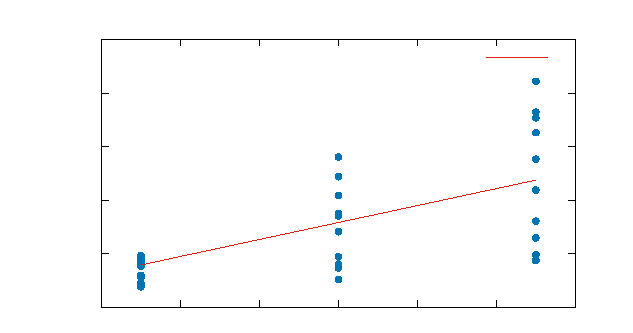
\includegraphics[width={288.00bp},height={144.00bp}]{brown_Ls}}%
    \gplfronttext
  \end{picture}%
\endgroup

    \caption{}
\end{figure}

\section{Závěr}

\begin{thebibliography}{0}
\bibitem{tabulky} Návod k úloze ~\url{https://www.physics.muni.cz/praktika/static/navody/fp2/uloha04.pdf}.   
\end{thebibliography}

\end{document}
